\documentclass{article}
\usepackage{hyperref}
\usepackage{amsmath,amssymb}
\usepackage{graphicx}
\usepackage{caption}
\usepackage{subcaption}
\usepackage{color}
\usepackage[section]{placeins}
\renewcommand{\thesubsection}{\thesection.\alph{subsection}}
\usepackage{listings}

\title{\bf{Combustion Exam}}
\author{Nicholas Malaya\\ Department of Mechanical Engineering \\
University of Texas at Austin}  
\date{}

\begin{document}
\maketitle

\newpage
\section*{Problem 1}
Consider a concentric spherical porous burner through which a pure
gaseous fuel enters through the inner sphere ($r_i$) and oxidant enters
through the outer sphere ($r_0$). Assume that the mass averaged velocity
in the system is zero and that the fuel and air diffuse from the walls
and are maintained at the walls with a mass fraction of unity. The walls
are a sink to the products and they disappear at the wall. A schematic
of the arrangement is shown in figure 1 below. 

\begin{figure}[h]
 \begin{center}
  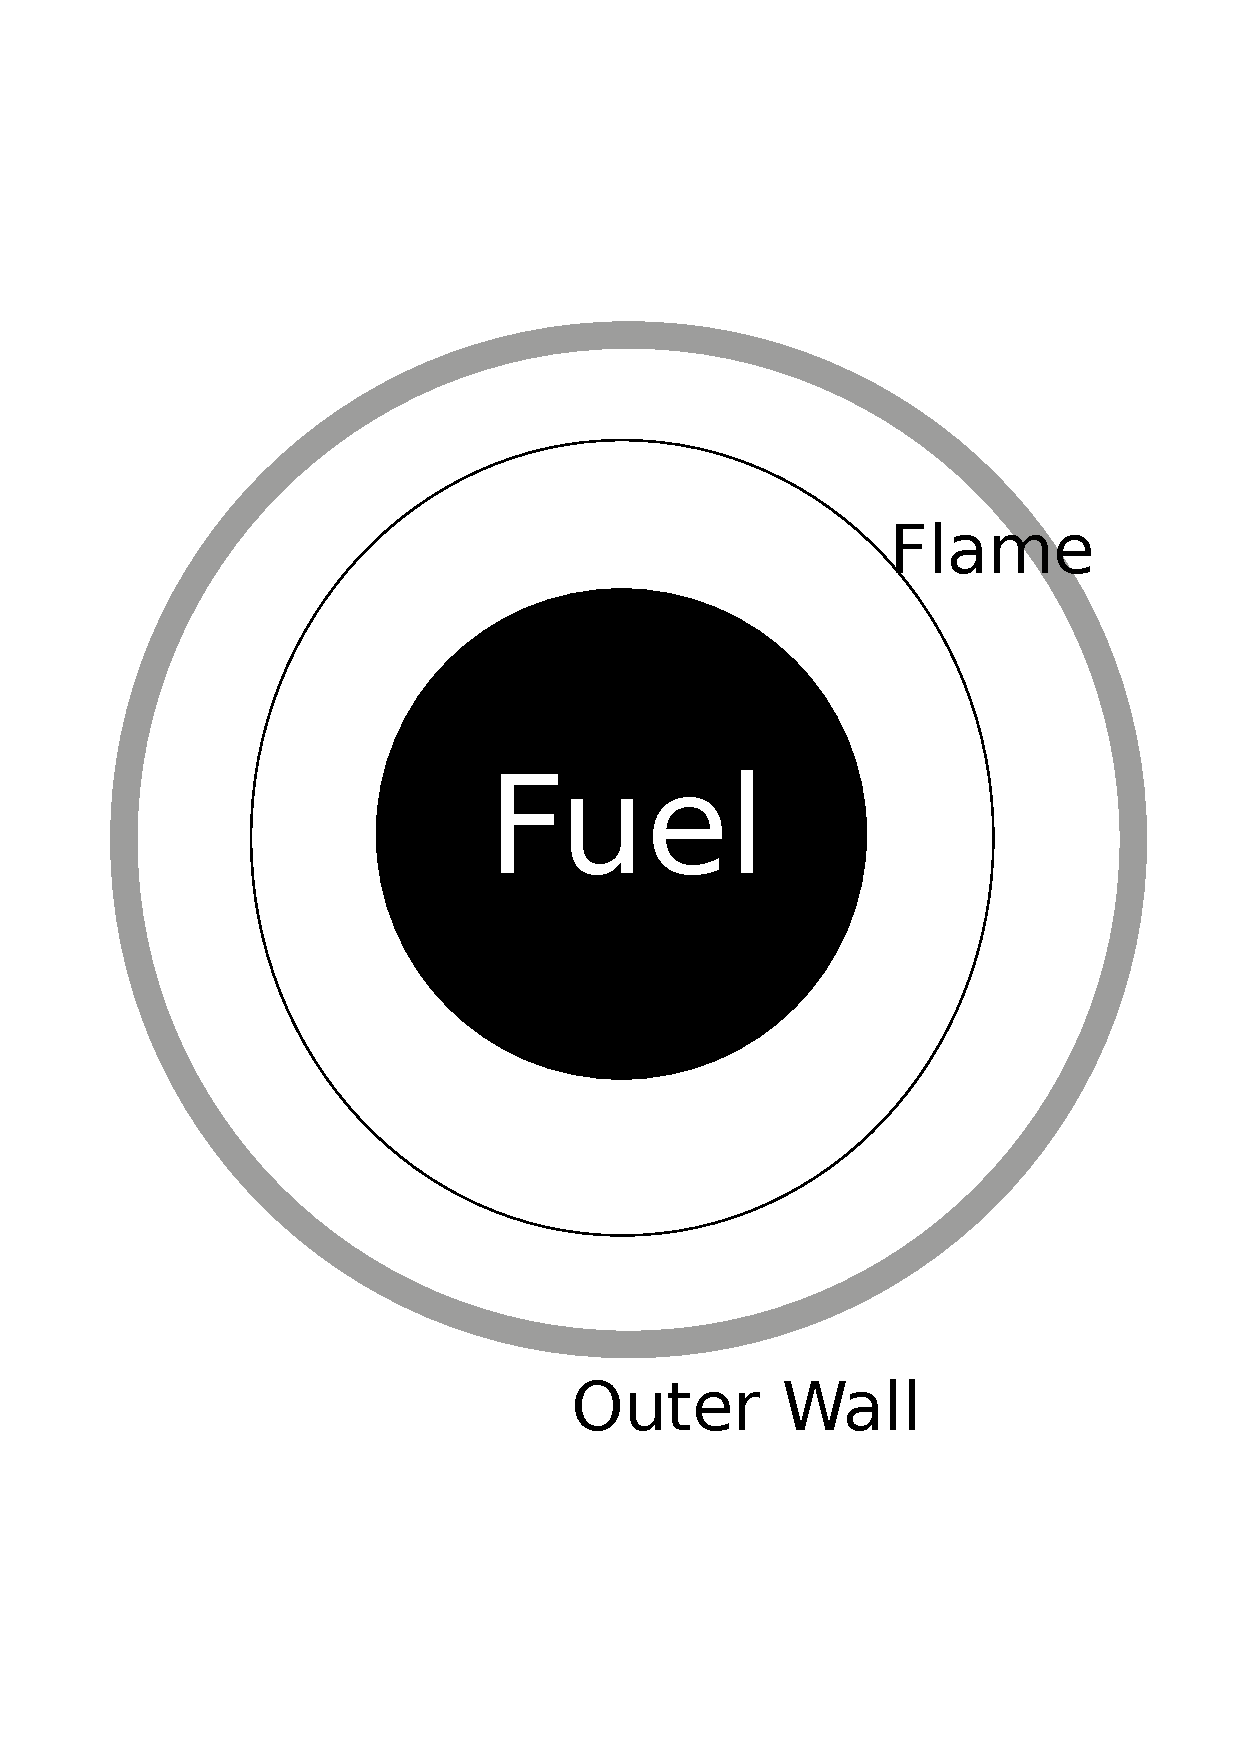
\includegraphics[scale=.3]{figs/spherical_burner.pdf}
  \caption{The spherical burner apparatus.}
 \end{center}
\end{figure}

The governing equation for the fuel is assumed to be, 
\begin{equation*}
 \frac{d}{dr}\left( r^2 \rho D \frac{dY_i}{dr}\right) = \pm r^2 w_i. 
\end{equation*}
Where, 
\begin{equation*}
 w_f = A Y_f Y_o e^{-E/RT}.
\end{equation*}
\begin{center}
\line(1,0){350}
\end{center}
\subsection*{a) How does the fuel mass fraction ($Y_i$) vary functionally
  with radius?}
We solve this spherical diffusion flame problem as a quasi-steady
problem, in that we assume the fuel at the center is not shrinking as a
function of time. Note that, 
\begin{equation*}
\omega = \frac{\omega_i}{\nu_i W_i}= \frac{\omega_F}{\nu_F W_F} =
 \frac{\omega_O}{\nu_O W_O} 
\end{equation*}
This hints at a conserved scalar form that will
decouple the chemistry from the convection-diffusion of a conserved
scalar quantity. In particular, 
\begin{equation*}
\mathcal{L}\left(\beta \right) = \mathcal{L}\left( \frac{Y_O}{\nu_O W_O}
	    - \frac{Y_F}{\nu_F W_F} \right) \Rightarrow \frac{d}{dr}\left( r^2
	    \rho D \frac{d \beta}{dr}\right) = 0 .
\end{equation*}
Now, we must solve this equation. After the first integration, we have, 
\begin{equation*}
\frac{d \beta}{dr} = \frac{C_1}{r^2 }.
\end{equation*}
This assumes constant density and transport properties. The second
integration in $r$ leaves us with, 
\begin{equation*}
\beta(r) = C_2 - \frac{C_1}{ r }.
\end{equation*}
In other words, $Y_i \propto \frac{1}{r} $. 

One comment: the boundary conditions are stated as, ``the fuel and air
 diffuse from the walls and are maintained at the walls with mass
 fraction of unity''. In other words, $B(r_i) \rightarrow Y_{F,i} = 1, Y_{O,i} =
 0 $ and $B(r_o) \rightarrow Y_{F,i} = 0, Y_{O,o} = 1$. 

\subsection*{b) How does the temperature vary functionally with radius?}

The $\beta$ in part a is not unique. We can also form a conserved scalar
quantity by defining $\beta = T + Y_i$. This results in precisely the
same conserved scalar differential equation form, 
\begin{equation*}
\mathcal{L}\left(\beta \right) = \mathcal{L}\left( \frac{Y_O}{\nu_O W_O}
	    - \frac{Y_F}{\nu_F W_F} \right) \Rightarrow \frac{d}{dr}\left( r^2
	    \rho D \frac{d \beta}{dr}\right) = 0 .
\end{equation*}
With an identical solution, aside from different constants of
integation,
\begin{equation*}
\beta(r) = C'_2 - \frac{C'_1}{ r }.
\end{equation*}
We assume that the Damkohler number is sufficiently large that there is
no (or at least, negligible) reaction leakage across the flame
sheet. This is a statement that $Da \rightarrow \infty$ in, 
\begin{equation*}
 \mathcal{\hat L}\left(\beta \right) = \text{Da } Y_f Y_O e^{-E/RT}
\end{equation*}
Where $\mathcal{\hat L}\left( \right)$ is the non-dimensional form of
the operator. This means we are assuming that the reactions are
infinitely fast (in comparison to diffusion in the fluid) and therefore,
the flame sits at an asymptotically thin region (a flame sheet) where it instantly
consumes any reactants.

The Shvab-Zel'dovich form is then,
\begin{eqnarray*}
 \beta_F(r) = T + Y_F = C'_2 - \frac{C'_1}{ r } \\
 \beta_O(r) = T + Y_O = C'_2 - \frac{C'_1}{ r }
\end{eqnarray*}
As a consequence of no reaction leakage, 
\begin{eqnarray*}
 Y_F = 0 \text{ when } r_f < r < r_o \\
 Y_O = 0 \text{ when } r_i < r < r_f \\
\end{eqnarray*}
Evaluating in these regimes then implies that the functional form of
temperature must therefore also be,  
\begin{eqnarray*}
 T = k - \frac{k}{ r } 
\end{eqnarray*}
Where k is yet another constant of integration. In other words, $T
\propto \frac{1}{r} $.  

\newpage
%\subsection*{c) Sketch the temperature, fuel and oxidant mass
%fractions.}
\subsection*{d) At what value of the radius does the flame sit?}

\begin{eqnarray*}
 r_f &= \left(\frac{Y_{F,i}}{Y_{F,i} + Y_{O,o}} \right)(r_o - r_i) + r_i \\
     &= \left(\frac{1}{1 + Y_{O,o}} \right)(r_o - r_i) + r_i \\
     &= \left(\frac{1}{1 + b} \right)(r_o - r_i) + r_i 
\end{eqnarray*}
Where b is the amount of oxidizer in the reaction. In the event that
$b=1$, then the reaction is stochiometric, and the flame will sit at a
distance halfway between the fuel and oxidizer sources. 

\newpage
\section*{Problem 2}



\end{document}
